\subsection{MVC-mønsteret}\label{MVC}

Et af de standardiserede design mønstre, som bruges af mange udviklere er MVC-mønstret - som står for \textit{Model-View-Controller}, en figur over modellen kan ses på \myref{MVC-Figure}.
MVC-mønsteret har til formål, at dele systemet op i tre komponenter, \textit{Model}, \textit{View} og \textit{Controller}.
Denne segregering adskiller således forretnings-logik, input-logik og UI-logik, og gør herved systemet mere fleksibelt, samt fremmer muligheden for at udvikle parallelt på de forskellige komponenter.
Dette kan være nyttigt i udviklingen af systemet, men også efter udgivelsen, idet blandt andet UI-logik kan blive ændret oftere end for eksempel forretnings-logik.
Opdelingen hjælper også til at skabe overblik over koden, og gør det nemmere at unit teste systemet via dets controllere. \citep{MVC_Overview}

Nedenfor beskrives de tre komponenter.

\textbf{Model}\\
Objekterne der udgør model-laget indeholder forretnings-logik, samt alle data der skal modelleres i systemet.

\begin{wrapfigure}{r}{0.4\textwidth}
	\vspace{0pt}
	\begin{center}
		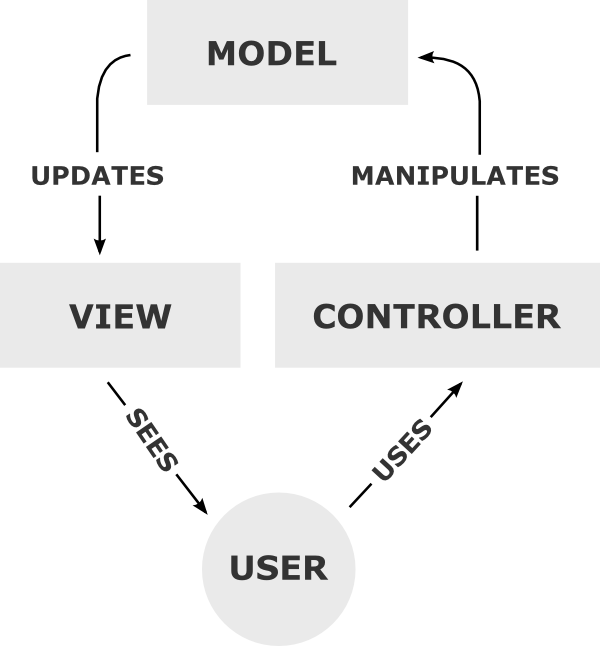
\includegraphics[width=0.38\textwidth]{images/Images/mvc.png}
	\end{center}
	\vspace{-20pt}
	\label{MVC-Figure}
	\caption{MVC-mønsteret \citep{mvcpic}}
	\vspace{-30pt}
\end{wrapfigure}

\textbf{View}\\
Det er igennem forskellige views, at brugeren får præsenteret brugergrænsefladen. 
Derfor giver det også mening, at placere UI-logik i denne del af MVC-mønsteret.
Indholdet i et view genereres ud fra data fra modellen.
Et eksempel på dette ville være visning af en liste af objekter ud fra en model, der indeholder netop en liste.

\textbf{Controller}\\
Controlleren håndterer interaktionen mellem brugeren og systemet.
Derfor er det også i de forskellige controllerer, at vi finder input-logikken. 
Her bestemmes ud fra input fra brugeren, hvilket data der skal arbejdes med i hvilken model og hvilket view, der skal præsenteres for brugeren.

